
\documentclass[journal]{IEEEtran}

\ifCLASSINFOpdf
   \usepackage[pdftex]{graphicx}
\else

\fi
%encoding
\usepackage{fancybox}
%--------------------------------------
\usepackage[utf8]{inputenc}
\usepackage[T1]{fontenc}
\usepackage{pgfplots}
\usepackage{subfig}
% Define o caminho das figuras

\usepackage{nomencl}
\usepackage{hyphenat}
\hyphenation{op-tical net-works semi-conduc-tor}

%--------------------------------------
 
%Portuguese-specific commands
%--------------------------------------
\usepackage[portuguese]{babel}
%--------------------------------------
 
%Hyphenation rules
%--------------------------------------
\usepackage{hyphenat}
\hyphenation{mate-mática recu-perar}
%--------------------------------------
\usepackage{graphicx}
\usepackage{placeins}
\usepackage{balance}
\usepackage{color,graphicx}

\begin{document}

\title{An Automated Testing Environment For The ITU-I/ISO-IEC Reference Video Codecs}

\author{\IEEEauthorblockN{	José Raimundo Barbosa\IEEEauthorrefmark{1}, 
							Jean Felipe Fonseca de Oliveira\IEEEauthorrefmark{3}
							Carlos Danilo Miranda Regis\IEEEauthorrefmark{1},
							Ruan Delgado Gomes\IEEEauthorrefmark{2}}
							
\IEEEauthorblockA{\IEEEauthorrefmark{1}Instituto Federal da Paraíba - João Pessoa\\}
\IEEEauthorblockA{\IEEEauthorrefmark{2}Instituto Federal da Paraíba - Guarabira\\}
\IEEEauthorblockA{\IEEEauthorrefmark{3}TPV Technology, São Paulo, Brasil}
\\E-mail:  jraimundo@lavid.ufpb.br, jeanfelipefonseca@gmail.com, danilo.regis@ifpb.edu.br, ruan.gomes@ifpb.edu.br
}


\maketitle
\begin{abstract}

H.265/HEVC is the state-of-the-art video codec, focusing in Ultra-High Definition video (UHD) and it is 50\% more efficient in bit-rate compression than its predecessor, the H.264/AVC. However this efficiency requires a high computational cost, which may compromise the use of the encoder in limited machines or in real time applications that use UHD videos. Several studies look for ways to enhance the HEVC encoder and reduce the computational cost. However, to develop optimized versions of the encoder it is necessary to perform tests that can last for hours and usually requires manual collection of coding information.  In this work, a tool to perform automated tests of HEVC encoders  was developed. The tool was implemented in a parallel architecture that allows the execution of several instances of the encoder. \textcolor{red}{It collect the informations and executes objective metrics to evaluate the efficiency of the encoder, the dualty of the encoder video and the encoding time. This work intends to provide a useful solution to help analyze encoders in long sequences of tests}.

\end{abstract}


\section{Introduction}


Currently, about three-quarters of annual data traffic on the Internet is assigned to video content, according to Cisco's Visual Networking Index report. In 2014 this consumption was 64\% and in 2020 this value will be about 80\%~\cite{Cisco:16}. One of the contributing factors is the increasing in video quality, which enables new experiences on Internet-broadcast television channels, video conferencing and on-demand video transmission services such as YouTube and Netflix, which already distribute videos in UHD~\cite{cheon:14}.


The UHD videos are \textcolor{red}{highly popular} in the market, because high pixel improve the perception of image details, allowing new experiences for viewers~\cite{cheon:14}. UHD 4K videos, for example, have resolution of 4096x2160 pixels while previous standards such as Full HD have 1920x1080. However, a raw UHD 4K stream, with 24 bits per pixel and 24 frames per second, requires a bandwidth of 5 Gbit/s~\cite{gomes:13}. These settings represent challenges in the storage and transmission of such videos.

To enable the intense and growing traffic of videos on the Internet and to satisfy the bandwidth conditions related to the UHD characteristics, it is necessary to develop codecs capable of a reducing the storage space and according data volume to bandwidth limitations~\cite{oliveira:16}\cite{wang:13}.  \textcolor{red}{However, when compression occurs several times or in the wrong way, it generates loss of information that can degrade image quality~\cite{netflix:16}}. In this context, the challenge arises of developing codecs capable of meeting the demand for UHD videos, and improving compression efficiency and image quality.

The ITU-T H.265~\cite{itu:265}, also known as High Efficiency Video Coding (HEVC), is the state-of-the-art codec which focus primarily on the newest UHD video technologies and presents a compression efficiency 50\% higher than its predecessor, H.264/Advanced Video Coding (AVC)~\cite{Bossen:12}\cite{Hanhart:12}\cite{Sullivan:12}. However, the encoder has a computational cost up to four times higher than H.264. This is attributed to the processing of the new block structures used in the compression, presenting challenges for situations that demand real-time video reproduction or in machines with processing limited processing power~\cite{Yoon:13}\cite{Correa:12}.


To promote HEVC optimization research, JCT-VC provided the HM reference encoder which features a implementation of HEVC that makes possible  to carry out studies on the efficiency of the codec and develop new features and optimizations~\cite{itu:10}. However, the comparison of performance of codecs developed based on the HM reference source code is a time-consuming process, since each test implies in the execution of several instances of the evaluated encoder and the reference encoder, which can last for several hours. After execution, is necessary to compare the UHD videos using objective or subjective metrics. With the comparisons it is possible to monitor the efficiency and performance of the new encoders compared to stable versions porposed scenario~\cite{netflix:16}.

This paper describes a tool for automated testing of HM based encoders. The tool was implemented in a parallel architecture in which multiple instances of the encoder are executed simultaneously. To calculate the encoder efficiency and the difference between the codecs, the Bjontegaard metric is used. This metric determines the difference of the efficiency of the codecs from the calculation of the mean difference of two curves adjusted by four points~\cite{Bjontegaard:01}, For the formulation of the standardized test cases, the recommendations of JCT-VC were followed~\cite{Bossen:15}. With the tool the comparison between the~\cite{oliveira:16} codec and reference codec~\cite{itu:10} was obtained and reduction of the test time by 86\% in a simple test case was verified, in which one video and one configuration were used, totalizing the execution of 8 instances.
	
	
%\section{Proposed test scenario}
\section{Standardization of Tests}	
%\subsection{Reference Codec HM}



The Joint Collaborative Team on Video Coding (JCT-VC) provided the open source HM reference encoder, which offers a implementation of HEVC in C++~\cite{Bossen:15}.The HM code provides an environment for the development of new features or optimizations, such as those developed in~\cite{oliveira:16},~\cite{Yoon:13},~\cite{Correa:12} and~\cite{Weerakkody:14}. In conjunction with the encoder, JCT-VC also provides the recommended settings and videos for standardized test suites. These settings will be presented later.

After encoding, HM generates, in addition to the encoded video, a record file containing important information about the encoding process such as bit rate, total encoding time, output video file size and PSNR for each YUV color matrix (Y = Luma, U = Chroma Blue and V = Chroma Red).


The way the tool was developed also enables to perform tests with the Joint Exploration Model (JEM) reference encoder~\cite{Bossen:17}. This encoder was developed based on HM and was presented in~\cite{JVET:2015} as the future of the environment for standardized development of HEVC video compression technology, including its current extensions and near-term extensions for screen content coding and high-dynamic-range coding.


%\subsection{Standardization of Tests}

To ensure common testing conditions, the JCT-VC committee has developed the JCTVC-L1100 documentation~\cite{Bossen:13}, which describes the settings and contents for standardized tests that explore different situations. This standardization is applied in the development of new features or encoder optimizations developed using HM. The settings discussed in the document are:

\begin{itemize}

  \item All Intra: All frames are encoded independently with only intra-frame prediction.
  \item Random Access (RA): Coding with high rates of compression compression. The coding order and the output order of the frames differ, inducing a coding delay. This setting represents broadcast and streaming applications.
  \item Low Delay P (LP): Coding without the structural coding delay presented when using RA parameters. This configuration is evaluated using only P-frames (uni-directional prediction).
  \item Low Delay B (LB): Similar to LP scenarios, but this configuration is evaluated using only B-frames, (unidirectional and bidirectional prediction).

\end{itemize}

These settings specify situations with videos with 8 bits per color component, configurations with 10 bits per color component aree also specified. In the documentation, the videos present in \emph{ftp://hevc@ftp.tnt.uni-hannover.de/testsequences/} are also recommended, requiring a registration to access the videos. Finally, the quantization values are specified: 22, 27, 32 and 37. In the tool, these values are already configured with standards, but it is possible to add more quantization values.

\section{Objective Metrics}

The evaluation of the quality of the videos can be carried out subjectively, that is, from the human evaluation \cite{itu:99}. However, this type of evaluation may be ineffective in detecting small image debris, which is generally difficult to perceive in the human eye, and may be exhaustive in long applications or in the case of real-time evaluation \cite{estrada:09}\cite{regis:12}. However, objective video evaluation techniques work better because they are faster and lower cost and indicate the existence of slight degradations \cite{regis:12}.

In this section, the objective metrics used in this work will be discussed.

\subsection{PSNR Metric}

The Peak Signal to Noise Ratio (PSNR) is one of the most used because of the ease of calculation and the low computational cost \cite{danilo:15}. This method expresses the maximum ratio of a signal and the noise of this signal and is constantly used to measure the structural quality of images. For this it is necessary to formulate the mean square error in addition to the digital representation of monochromatic images I and K of size m x n, the MSE is defined by the equation \ref{mse}.

\begin{equation}
	\centering
	\label{mse}
	MSE=\frac{1}{mn}\sum_{i=0}^{m-1}\sum_{j=0}^{n-1}[I(i,j)-K(i,j)]^{2}
\end{equation}

In this way, the PSNR is represented by \ref{psnr}, where MAX indicates the maximum possible pixel value in an image.

\begin{equation}
	\centering
	\label{psnr}
	PSNR = 10 \cdot log_{10}(\frac{MAX^{2}_{I}}{MSE}) = 20 \cdot log_{10}(\frac{MAX_{I}}{\sqrt{MSE}})  
\end{equation}

\textcolor{red}{
The higher the ratio of signal power to noise power the better the quality. For example: PSNR values (in decibels) above 42dB correspond to compressions that introduce imperceptible losses to the human eye, which means exceptional quality. We can consider videos with PSNR above 36dB is quite acceptable quality, between 30dB and 36dB we will have a medium quality and below 30dB the quality is already bad.
}

\subsection{SSIM Metric}


The Structural Similarity Index (SSIM) is a consolidated and constantly used model for video quality comparison. It is based on the assumption that the human visual system is highly adapted to extract structural information from images~\cite{danilo:12}. \textcolor{red}{ Therefore, each pixel has a strong dependence on the others and this dependence increases with the proximity. This dependence presents important information about the structure of the objects in the image and that quantifying the structural change of an image can provide a good approximation to the perceived quality~\cite{Wang:02}.}

To identify the structural information, the SSIM metric uses a statistical approach based on the average luminance and $n \cdot n$ block contrast of the image. The mean ($\mu$), standard deviation ($\sigma^{2}$) and covariance ($\sigma_{fg}$) are calculated for each block. The mean and standard deviation are approximate estimates of the luminance and contrast of the image, respectively. Covariance is the measure of how much a signal is different from the other.

SSIM uses the measure of structural distortion rather than the error itself. If $x = \{x i | i = 1, 2,. . . , N\}$ represents the original signal and $y = \{y i | i = 1, 2,. . . , N\}$ represents the distorted signal, where i is the pixel index value. The structural similarity index can be calculated according to the equation \ref{ssim} ~\cite{oliveira:16}\cite{Wang:02}.

\begin{equation}
\label{ssim}
\centering
SSIM(x, y) = \frac{(2\mu _{x}\mu _{y} + c _{1})(2\sigma _{xy}+c _{2})}{(\mu_{x}^{2}+\mu_{y}^{2}+ c_{1})(\sigma _{x}^{2}+\sigma _{y}^{2}+c _{2})}
\end{equation}


\textcolor{red}{
In the Equation \ref{ssim},  $\mu_{x}$ represents the average of x,  $\mu_{y}$ represents the average of y. The variance of x is represented by $\sigma _{x}^{2}$ and the variance of y by $\sigma _{y}^{2}$. The $c_{1}=(k_{1}L)^{2}$, $c_{2}=(k_{2}L)^{2}$ are the variables to stabilize the division with weak, watch $L = 2^{n} - 1$ is the dynamic range of bits and $k_{1}=0.01$ and $k_{2}=0.03$ by default.
}





\subsection{PW-SSIM Metric}

The Perceptual Weighting Structural Similarity Index (PW-SSIM) uses a weighting-based approach to evaluate image quality, giving more importance to visually more important regions \cite{danilo:15a}. For this the magnitude of the gradient vectors of the original video is calculated using Sobel masks \cite{furnari:15}, then a frame is generated in which the pixel values are the magnitudes of the gradients. Then, this frame is partitioned into blocks of $8 x 8$ pixels and for each block is calculated the Spatial Perceptual Information (SI) \cite{jean:15}. The SI is expressed by Equation \ref{si}.


%\Delta R = \frac{R_{B}(D) - R_{A}(D)}{R_{A}(D)}

%\Delta R = 10^{r_{B}{(D)}-r_{B}{(D)}}-1
\begin{equation}
	\centering
	\label{si}
	SI = \left ( \frac{1}{N-1}\sum_{i=1}^{1}(\mu_{S}-S)^{2} \right )^{\frac{1}{2}}
\end{equation}

Where $N$ is the number of block and $\mu_{S}$ represents the average magnitude of the gradient in a block.

\begin{equation}
	\centering
	\label{pwssim}
	PWSSIM(f,h)= \frac{\sum_{d=1}^{D}SSIM_{d}(f,h)\cdot SI_{d}}{\sum_{d=1}^{D}SI_{d}}		
\end{equation}

Where $D$ is the distance of the object, and $f$ is the representation of a 2D video and $h$ represents a 2D video degraded.


\subsection{Bjontegaard Metric}

The Bjontegaard metric is considered the state-of-the-art with regards to the evaluation of video coding mechanisms and is one of the most widespread metrics in the current literature~\cite{Bjontegaard:01}\cite{Mathias}. It allows to obtain the values for overall bit rate (BD-Rate) in percent for two different encoding algorithms
considering the same PSNR or overall video quality difference (BD-PSNR) for two different encoding algorithms considering the same bit rate. %These values are used to evaluate the efficiency of the modified encoders in relation to the HM reference encoder.
	
The BD-PSNR is the measure corresponding to the average difference of Peak Signal-to-Night Ratio (PSNR) in decibels, between two encoders, considering the same bit rate. The BD-Rate value corresponds to the average percentage bit difference for the two encoders. In this work, more attention was given to bit rate and time evaluation.	


In~\cite{Mathias}, it is exemplifies the BD-Rate by means of Figure~\ref{fig:chart_barate}, where the curves are further drawn by linear interpolation. For the BD calculations, the rate axis is logarithmized and the rate-distortion curves are interpolated by an advanced interpolation method. The overlapping portions of the rate-distortion curves are used for calculation of the BD values. Depending on the range of overlap of the two curves, the resulting BD measurements get more or less meaningful. Therefore, a careful interpretation of the resulting numbers is required.


\FloatBarrier
\begin{figure}[!ht]
	\centering
	\caption{Interpolation of the BD-Rate \cite{Mathias}.}
	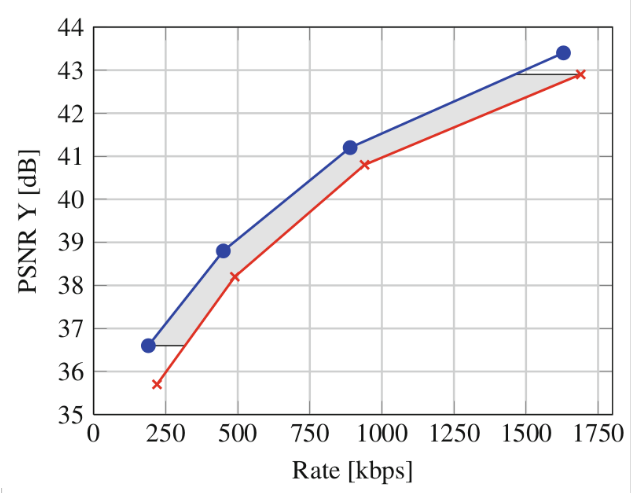
\includegraphics[width=0.4\textwidth]{figures/chartbdrate.png}
	\label{fig:chart_barate}
\end{figure}
\FloatBarrier
	

\section{Related Works}


In the literature it is possible to find several studies related to HEVC optimization techniques. Usually the methodological characteristics used in the development of the new technique as metrics and videos used are presented, besides the obtained results. However the test stage is vaguely mentioned or simply has its description ignored. As it happens in~\cite{oliveira:16}, an alternative is presented that uses machine learning to predict the partitioning of the macroblocks and to avoid the extra processing, and the proposed solution is compared with the HM reference encoder. In~\cite{Wang:16}, a parallel approach is used to accelerate coding by distributing multi-core processor efforts. And in~\cite{wang:13}, it is proposed an optimized partitioning algorithm, which refer to a scenario where the coded videos are processed by metrics and then the results are compared, without the aid of a tool for extraction and calculation.


The alternative proposed in~\cite{msu:16} offers a encoder comparison service, in which several configurations are predefined for the tests. For this it is necessary to submit the encoder to one of the paid services offered. Considering the best service, the premium, includes the SSIM, PSNR objective metrics and subjective metrics psycho visual enhancements, also includes the configurations High Speed, Normal and High. Quality, and presets analysis of systhetic motion, distortion in tail area and spatially variable noise. However, this alternative requires payment for more complex tests and also limits testing to a fixed number of configurations and test cases, nor is more current and advanced metrics like BD-Rate and BD-PSNR mentioned. The postponed solution also uses as reference encoders implemented based on X.265, for UHD video tests, this encoder is constantly mentioned in the literature, however the test scenarios proposed by the JVET specify HM encoders, these specifications help to standardize and document studies on the enhancement of the HEVC encoder.


\section{Tool Description}

To verify the efficiency it is necessary to perform several tests in which the modified encoder is executed in several coding scenarios, and then the results of each coding are compared with the results of the reference encoder. Each test sequence of an encoder can last for hours, depending on the videos and test settings, which hinders the development stage. The comparison is made between values such as bit rate, PSNR, coding time, and so on. These values are generated automatically by the HM encoder and are saved in log files. However, for their use it is necessary to manually collect in each log file which a repetitive work and can result in errors from human failure. 

The tool developed in this work executes instances of the modified encoder and reference encoder in all required configurations and then automatically collects all the information necessary for the comparison. With the data collected from the log files the calculation of the Bjontegaard \cite{Bjontegaard} metric is performed. The tool architecture can be viewed in Figure \ref{fig:fluxo}. The modular architecture of the tool enables other metrics to make use of the encoding values. To reduce the time of the tests, the tool was implemented in a parallel architecture in which multiple instances of the encoder are executed simultaneously, thus considerably reducing the time of a test.
%%usar a mesma fonte do texto
\FloatBarrier
\begin{figure}[!ht]
	\centering
	\caption{Tool architecture.}
	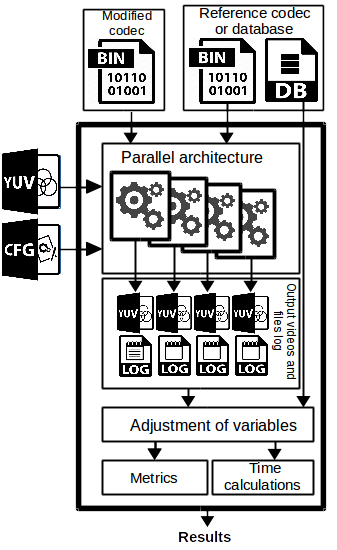
\includegraphics[width=0.4\textwidth]{figures/fluxo.png}
	\label{fig:fluxo}	
\end{figure}
\FloatBarrier

To prevent data loss during an unexpectedly stopped execution, a tool log file is generated that saves the current state of the test and makes it possible to return from where it left off. It is also possible to save the data of the tests performed by the encoders, thus avoiding to repeat the process and thus to promote the construction of a database with the results of the tests.

To execute the tests, the tool receives the parameters specified in Table \ref{parameter_tool}, these parameters indicate the settings that will be addressed equally by the modified encoder and the reference encoder that will generate different outputs. If the parameters are not informed, default values will be used that will execute the tool using a CIF video (352x288) and a one of the standard settings (Random Access Encoding). These parameters have minimum specifications only for checking the operation of the tool. It is important to check the memory and thread limitations before running the tool, it is recommended to run one thread for every two GBs of RAM. In case of an unexpected interruption, the execution of the tool with the -bkp flag activates the backup and the test will return to the moment of interruption.

\FloatBarrier

\begin{table}[!ht]

\centering
\caption{Parameters for tool execution.}
\label{parameter_tool}
\renewcommand*{\arraystretch}{1.5}
\small
\begin{tabular}{|l|l|p{4cm}|l|}
\hline
\textbf{Command} & \textbf{Example}      & \textbf{Description}                                         \\ \hline
./CodecTest      & --                    & Tool executable                                                             \\ \hline
-thr             & 2                     & Number of threads                                            \\ \hline
-vin             & 1 path/video.yuv  & Number of video followed by the video files                  \\ \hline
-cfg             & 1 path/File.cfg & Number of configuration followed by the configurations files \\ \hline
-outl            & path/out/logs/      & Path where log files will go                                 \\ \hline
-outv            & path/outvideos/    & Path where encoded videos will go                            \\ \hline
-eva             & path/BinEncoder    & Rated encoder binary                                         \\ \hline
-ref             & path/BinEncoder    & Reference encoder binary                                     \\ \hline
-fr              & 30                    & Frame rate                                                   \\ \hline
-f               & 130                   & Number of frames                                             \\ \hline
-q             	 & 4 22 27 32 37        & Number of quantization followed by the quantization values   \\ 
\hline
-wdt             & 3840                  & Video width                                                  \\ \hline
-hgt             & 2160                  & Video height                                                 \\ \hline
-bkp             & --                    & Backup flag                                                  \\ \hline
\end{tabular}
\end{table}
\FloatBarrier

The output file structure of the testing tool presents the key information about the execution of each instance, in addition to the total time values and the values of the metrics. A log file example is shown in Figure \ref{fig:log}.

\FloatBarrier

\begin{figure}[!ht]
	\centering
	\caption{File log example.}
	\fbox{
	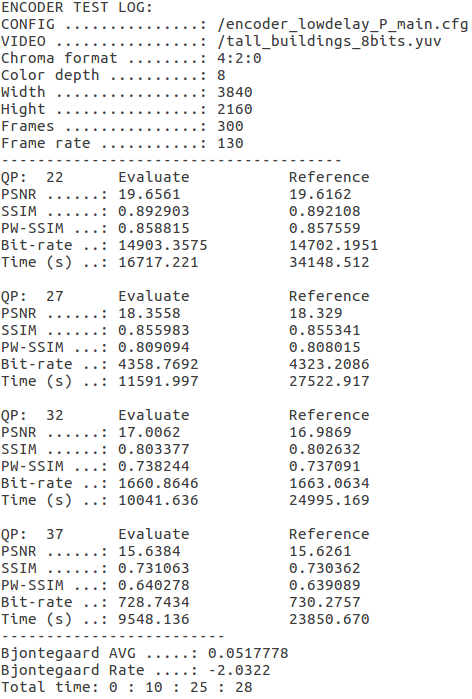
\includegraphics[width=0.4\textwidth]{figures/log.png}
	}
	\label{fig:log}
\end{figure}

\FloatBarrier

For more complex tests, the implementation of a distributed version of the tool is in progress, which will allow the execution of more instances of the encoder according to the configuration and quantity available machines. Online services are also being developed, in which researchers and developers can submit the executable program of their encoders and select the configurations so that the tests are performed on a robust server. With this proposal also intends to build a database fed with the data of the tests of the users, this database will contribute to other researchers.

It is also possible to observe the values of Bit Rate per QP used in the test in \ref{bitqp}, and also the PSNR values by QP in \ref{psnrqp}, these graphs are generated automatically after the tool execution.

\FloatBarrier
\begin{figure}[!htb]
	\centering
	\caption{Chart examples.}
	\subfloat[Bit Rate x QP.]{
		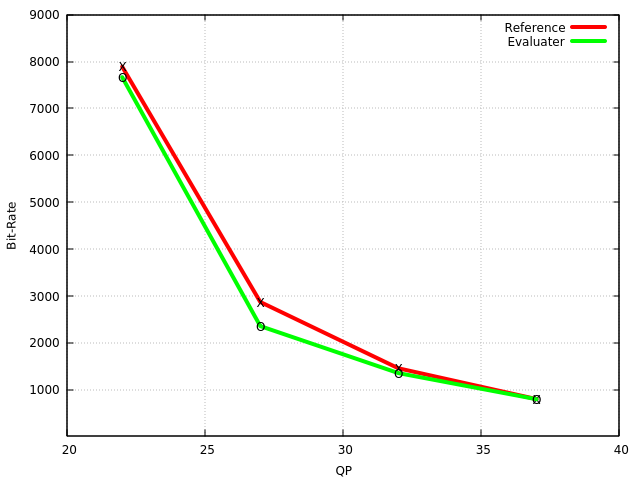
\includegraphics[height=5cm]{figures/bitrateqp.png}
		\label{bitqp}
	}
	\quad %espaco separador
	\subfloat[PSNR x QP.]{
		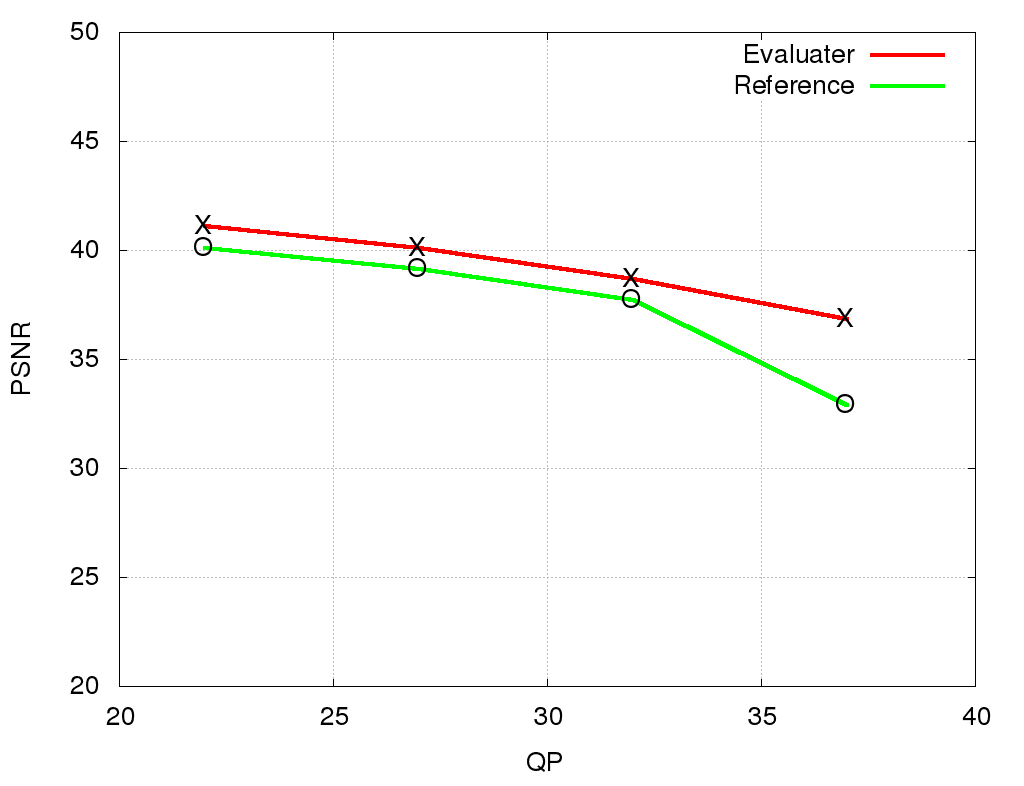
\includegraphics[height=5cm]{figures/psnrqp.png}
		\label{psnrqp}
	}
\end{figure}
\FloatBarrier

%---------------------------------------------------------	
	

%\pagebreak

\section{Result}

To validate the tool, a sequence of tests was performed to compare the encoder developed in REFERENCIA with the reference encoder HM.16. The tests were performed on a computer with processor SPECIFICATIONS. We used the UHD 4K videos available in REFERENCE. In total, N frames of X sequences were used, being SEQUENCNAME.


The total time spent executing the test sequence using the tool was considerably less than the test performed manually, ie running one encoder or more at a time, calculating the values of the metrics and documenting the results. Because it is an alternative with multi-threaded processing, time reduction is something that is already expected, but adequate management is required so that the execution of different threads does not compromise the integrity of the values used to calculate the metrics, time and other information present in the sequence of tests.


\bibliographystyle{waslon}
\bibliography{sample}


%\balancecolumns 

\end{document}